% !TEX root = manuscrit.tex

\chapter{Introduction}
	
%In this work, our aim is to investigate how formal methods can be applied in the context of mobile robot algorithms.

The tasks which may be performed by autonomous robots are increasingly numerous and complex, 
both in our everyday life or for industrial use.
Many investigations have been focusing recently on %distributed systems with autonomous mobile entities (called 
autonomous mobile robots %robots) capable of moving in a spatial environment and  
which must cooperate to achieve a common complex task that they cannot perform alone. 
Surveys can be found for instance in~\cite{Prencipe13, butucaru_distributed_2011,FPS12}. 
% without either any central control or any message passing based communication mechanism
Possible applications for such multi-robot systems include environmental monitoring, map construction, urban search and rescue, surface cleaning, surrounding or surveillance of risky areas, exploration of unknown environments, etc.
For example, such robots can patrol the docks in a harbor, as depicted in Figure~\ref{fig:port}.
\begin{figure}[h]
\begin{tikzpicture}[x=1em,y=1em,fill=blue!50]
  \pgfmatrix{rectangle}{center}{mymatrix}
    {\pgfusepath{}}{\pgfpointorigin}{}
    {
	\node[] at (0,0) {\includegraphics[scale=0.06]{robot}};
      \fill (1,-4)  rectangle (2,1);
      \fill (2,-3)  rectangle (3,0);%\atorig
	 \pgfmatrixnextcell
      \fill (-3,0)  rectangle (1,1);%\atorig2 
	 \pgfmatrixnextcell
      \fill (-1,-4) rectangle (0,-1);%\atorig3 
	 \pgfmatrixnextcell
      \fill (0,-1) rectangle (-1,-3);%\atorig4 
	 \pgfmatrixnextcell %ici pour un carré
      \fill (4,-3) rectangle (5,1);
      \fill (1,3.5) rectangle (6,2.5); 
      \fill (-1,0.5)  rectangle (4,1.5);%\atorig5
      \fill (3,-1) rectangle (4,-3);
	  \pgfmatrixnextcell 
	 \node[] at (-3,2) {\includegraphics[scale=0.06]{robot}};
      \fill (0,-1)  rectangle (2,0);%\atorig6 
      \fill (-2,-2) rectangle (0,-1);
	  \pgfmatrixnextcell
      \fill (0,0)   rectangle (1,-4);%\atorig7 
	  \pgfmatrixnextcell
\node[] at (-2,-3) {\includegraphics[scale=0.06]{robot}};
      \fill (1,-2) rectangle (2,2); \\
	   % \pgfmatrixnextcell
    }
\end{tikzpicture}
\caption{Robot example}
\label{fig:port}
\end{figure}
They must coordinate to keep away thieves from the cargo containers, by verifying regularly that no container has been opened. 
%Each robot must regularly ensure that each container is safe.
After chasing a thief outside the port, they have to drive back near containers that need the most to be checked.

Such a cooperating  team is called a distributed system \cite{Lynch96,Tel:2001:IDA:517021}. A system is distributed when it is composed of a set of autonomous computation entities endowed with communication abilities in order to solve a common task.
Traditionally, the entities have been assumed to be stationary and to communicate with each other thanks to message passing. 
The robot model we study in this thesis \cite{suzuki_distributed_1999,FPS12} differs from the classical one in two aspects: 
the entities are mobile and they do not communicate via message passing. Moreover, these mobile entities may be endowed with limited capabilities.
The concern in mobile robots research is to understand what kind of basic capabilities are needed for the robot team in order to accomplish a given task, in the absence of any central coordinating authority, and at what cost.
Several tasks have been investigated both in the plane or in a discrete environment.
Since these assigned tasks may be critical, it must be ensured that the robots accomplish them correctly, in spite of their limitations.

So far, robot networks have been either validated empirically or algorithm designers wrote handmade proofs. 
These proofs are hard to write and read, and reasoning on complex systems is both cumbersome and error-prone. 
Automated proofs on an abstract mathematical model of the system could remove the fastidious task of inspecting the system behavior to ensure its correctness with respect to a certain specification, \ie the definition of what  the system is expected to do, described by a set of properties.
Such techniques are called formal verification techniques.
Several approaches exist: 
\begin{description}
\item [Test\hfill] \index{Test} Test is probably the most frequently used method. In a first phase, execution scenarios whose results are known in advance have to be developed. The system is then executed in accordance with such a scenario and one can check if the output is as expected.
The presence of such tests does not guarantee the correctness of system behaviors outside the cases tested. Moreover, the design of adequate tests is more difficult for concurrent or distributed systems.
\item [Proofs\hfill] \index{Proof} In this approach, 
the semantics of a system (or a class of systems) is formalized in a mathematical language. Then the argument underlying a hand proof is formalized in the logic of a proof assistant and the proofs are checked mechanically.
Thus an expert user must interact to properly orient the proof construction. Besides, when a proof fails, the diagnostic is known to be difficult.
Various proof assistants have emerged since the 60’s: PVS\footnote{http://pvs.csl.sri.com}, Coq\footnote{https://coq.inria.fr/} and Isabelle/HOL\footnote{https://isabelle.in.tum.de} are among the most widely used.
\item [Model checking\hfill] \index{Model checking} The system and the properties to be verified must be first formalized, possibly abstracting away irrelevant details. An algorithm, which depends on the classes of models for the system and the properties, is then applied to check whether the properties are satisfied by the model. One advantage of this technique is its ability to extract behavior invalidating properties. Thus, it can be used at the design phase to validate prototypes. A drawback of this method is the so called combinatorial explosion: exploring all executions in a model of large size is time and memory consuming.
The model checkers \textsc{Uppaal}\footnote{http://www.uppaal.org} and \textsc{Spin}\footnote{http://spinroot.com/spin/whatispin.html} are amongst the most frequently used.
\end{description}
Each of these approaches has its strengths and drawbacks: While tests can be easy to implement, they cannot be applied in the design phase and the generation of exhaustive tests is a difficult problem; Proofs are difficult to implement since they require the presence of an expert, but they are exhaustive, applicable at the design phase, and
they can handle systems where some variables are not specified (like for instance the number of processes), called parameterized systems; 
Finally, the model checking approach is a comprehensive and automatic one but limited by the model size. 
Moreover, the problem is  undecidable in general for parameterized systems~\cite{apt.kozen.86}.


While the correctness of an algorithm can be verified at the design phase by model checking and assisted proof, 
another formal technique called synthesis aims at automatically generating a protocol from its specification. An advantage of this method is that the generated protocol is correct by design.
%The produced protocol is correct by designed.  
%Automatic synthesis is a more difficult problem since it produces a program that is . 
This question raised early interest~\cite{emersonclarke1981, MannaWolper84} and actually goes back to Church~\cite{Church62, BuchiLandweber69}. It is even more difficult when the program to generate is intended to work as an open system, maintaining an on-going interaction with a (partially) unknown environment. Given a specification, if there exists a program such that its behavior satisfies this specification, regardless of the environment behavior, then this program must be automatically built. Otherwise, it must be proved that the problem cannot be solved.

 It is known since \cite{BuchiLandweber69} that a successful approach consists in viewing the synthesis problem as a \emph{game} between the system and the environment. The system and its environment are considered as opposite players, the winning condition being the specification the system should fulfill. Then, the classical problem in game theory of determining winning strategies for the players is equivalent to finding how the system should act in any situation, in order to satisfy its specification, irrespective of how the environment behaves.
However, this problem is also undecidable in general for distributed systems~\cite{PnueliR90}. 
 \bigskip
 
 In this work, our aim is to investigate how formal methods can be applied in the context of mobile robot algorithms.
 We would like to bring out the benefits of these methods compared to traditional approaches.


\bigskip
%\todo{plan de l'intro}
In the next sections, we present the robot model considered in this manuscript, as well as existing work on the two main problems 
studied here: exploration and gathering by mobile robots. 
Then, we give a more detailed description of the formal methods devoted to the verification of mobile robots protocols. 



	\section{Mobile robots}
In this thesis, we consider a theoretic model \cite{suzuki_distributed_1999,FPS12}, where it is possible to express that robots with limited capabilities 
cooperate to achieve a common objective. 
In this model, each robot behavior is an infinite sequence of cycles where each cycle is divided into three phases: 
The Look phase, the Compute phase and the Move phase.  \index{Look-Compute-Move}
We first give a brief overview of these phases, restrictions are discussed in the next paragraph.
\begin{description}
\item [Look] The robot observes its environment ; the result of this operation is a snapshot of the positions of all robots within its radius of visibility with respect to its own coordinate system. 
\item [Compute] The robot executes the algorithm (the same for all robots), using the snapshot of the Look operation as input, the result is a  destination point given relatively to its coordinate system. 
 \item[Move] The robot moves toward the computed destination; if the destination is the current location, the robot stays still, performing a null movement. 
 \end{description}
 
This model called ATOM, also referred  in the literature as the SYm model, was proposed by Suzuki and Yamashita~\cite{suzuki_distributed_1999}.
 It was then refined by Prencipe~\cite{prencipe_new_2000} into a more realistic version called the CORDA model. 
 These models differ in their degrees of atomicity: 
\begin{itemize}%%%%%%%%%%%%%%%%%%%%%%%%%%%%%%%%%%%%%%%%%%here executes ? aver un subset ?
\item In the historical model, ATOM\index{ATOM}~\cite{suzuki_distributed_1999}, some non-empty subset of robots executes the three phases synchronously and atomically. This gives rise to two variants: Fsync, for the fully-synchronous model where all robots are scheduled at each cycle, and Ssync, for the semi-synchronous model, where a strict subset of robots can be scheduled. 

%Ssync
\index{Ssync}
In the semi-synchronous (Ssync) model, one or more robots are activated at each cycle, and obtain the snapshot corresponding to its observation, but all these snapshots are taken simultaneously and atomically. Based on that snapshot, they compute and perform their move. As a consequence, no robot will ever be observed while moving, and the understanding of the universe by the active robots is always consistent. In this case, the system behavior corresponds to executing all operations instantaneously (all Look/Compute operations immediately followed by all Move operations). 
%Note that such a system is equivalent to a synchronous system in which the chosen robots are activated simultaneously and all operations within a cycle are instantaneous. Indeed, the unpredictability is restricted to which robots are activated in each cycle (and the destination).
%Fsync
\index{Fsync}
The fully synchronous (Fsync) model is a particular case of Ssync, since in each cycle, all robots are activated. 
\item
The second model, CORDA~\cite{prencipe_new_2000}, \index{CORDA} also called Async\index{Async}, is a more realistic variant: In this less constrained model, each robot is activated asynchronously and independently from the other robots. Furthermore, the duration of each phase as well as the time between successive phases in the same cycle are finite but unknown. As a result, computations can be based on totally obsolete observations, taken arbitrarily far in the past. Another consequence is that robots can be seen while moving, creating further inconsistencies in robot views. 
\end{itemize}

A particular variant, between Async and Ssync, has been considered in~\cite{LinMA07a}. In this limited form of asynchrony, called partial Async, the time spent by a robot in the Look, and Compute phases is bounded by a globally predefined amount, while the time spent in the Move phase is bounded by a locally predefined quantity (not necessarily the same for each robot). 

Note that  in term of executions, Fsync is included in Ssync, and Ssync is included in Async.

\bigskip
The ability of a team to achieve an assigned task depends mainly on the capabilities of its robots:  the more powerful they are, 
the more easily the task is solved. %The concern in mobile robots research is to understand what kind of basic capabilities are needed for the robot team in order to accomplish a given task, in the absence of any central coordinating authority, and at what cost. 
 
%They are endowed with sensing, computing, and moving capabilities described below. 
\subsection{Robot weaknesses}
We now detail the minimal assumptions usually made on these robots.
%Anonymous and similar: 
\index{Anonymous}
The robots are identical and anonymous, they execute the same algorithm and they cannot be distinguished using their appearances, but they can have different computing speeds and different moving speeds (in the Async case). Robots may have identities but neither they nor the other robots have knowledge or access to these identities. 
%know or can have access to these, only an omniscient observer has this knowledge.

%oblivious
\index{Oblivious}
The robots are oblivious \ie they have no memory of their past actions. 
%their actions do not depend on previous actions. 
This capability implies that any state can be considered as initial. Hence, robot algorithms will have self-stabilization\index{self-stabilization} properties: 
A self-stabilizing distributed protocol ensures that a correct behavior can be recovered in a finite time without any external or manual help.
%In~\cite{DieudonneP12}, Dieudonne et Petit discuss on the link between the mobile robot model and self-stabilization.

%no common handiness: 
\index{handedness}
\index{chirality}
Robots  have neither a common sense of direction, nor a common handedness (chirality).
Each robot has its own unit of length and a local compass defining his own local Cartesian coordinate system. This local coordinate system is self-centric, \ie the origin is the robot's position. Moreover, the local coordinate system of oblivious robots may completely change during their life. However, it remains invariable during a cycle.

%no communication; other works communication: via msg, pebbles, ...
\index{Communication}
The robots are silent: there is no communication via message passing.
They communicate by observing other robots positions, and taking a decision accordingly. In other words, the only mean for a robot to send information to some other robot is to move and let the others observe.


\subsection{Robot capabilities}
To execute their Look-Compute-Move cycles, the robots are endowed with sensing, computing and moving capabilities. These capabilities 
depend on the environment that can be continuous or discrete.
%anissa
Two cases have been studied in the literature: 
\begin{itemize}
\item The continuous euclidean space \cite{suzuki_distributed_1999,FPS12}, in which the robots entities move on a plane, \index{Continuous space}
\item The discrete universe~\cite{KlasingMP06,flocchini_computing_2007}, in which space is represented by a graph, where nodes correspond to the possible locations and edges to the routes for a robot from one location to another.\index{Discrete space}
\end{itemize}
The discrete representation is motivated by practical aspects with respect to the unreliability of sensing devices used by the robots as well as inaccuracy of their motorization~\cite{CDDMJ08j}.  A discrete setting permits to approximate these features and simplify the design of robot models by reasoning on finite structures. However, it is more sensitive to the size of constants, which may significantly increase the number of symmetric configurations 
when the underlying graph is also symmetric (\emph{e.g.} a ring) and thus the size of correctness proofs~\cite{ASN11c, KLOT11, KLOT12}.


\subsubsection{The sensing capability}
\index{Visibility}
 Robots are endowed with visibility sensors providing the locations of other robots. The obtained location is either fine grained (which means that it has been obtained with some degree of accuracy) or coarse grained (robots can only be observed at some specific discrete locations, each location being adjacent to one another). In the first case, the literature mostly refers to the continuous space model, while in the latter case, it is the discrete one.
 
Robots are dimensionless and thus their visibility cannot be obstructed:  if three robots $r_1$, $r_2$, and $r_3$ are aligned, with $r_2$ in the middle, $r_1$ can see $r_3$. Moreover, robots may share the same position: this is called a \emph{multiplicity point} or a \emph{tower} \cite{FPS12}. The ability for a robot to detect multiplicity is crucial to achieve some particular tasks. We distinguish weak and strong multiplicity detection. 
\begin{itemize}
\item The weak multiplicity detector detects whether there is zero, one or more than one robot at a particular location. 
\item The strong multiplicity detector senses the exact number of robots at a particular location. 
\end{itemize}
This sensor may be local or global: in the local setting a robot only detects multiplicity at its current position, while in the  global setting the multiplicities of all positions are known by all robots.

A third characteristic of robot sensing capability is their visibility radius. It can be infinite \ie a robot is able to sense the position of all other robots, or finite \ie there exists a bound (expressed as a distance) beyond which a robot cannot sense anything.
Note that the sensing is defined in the robot’s own coordinate system.

\subsubsection{The computing capability}
As in classical distributed systems, robots are assumed to be able to perform any finite sequence of computing steps in negligible time. 
Since robots are oblivious, volatile memory is used to perform computing tasks in a single Look-Compute-Move cycle, but the memory content is erased at the end of each cycle.
The computation takes as input the observation made in the Look phase and gives the robot a move.
When two robots are on the same location or are symmetric, they should be given the same move.
In some instances, when the robot observation does not permit to distinguish directions, the computed location may be ambiguous: it then corresponds to a non deterministic move, which can be resolved by a scheduler.

\subsubsection{The moving capability}
Robots may move only to the location provided by the computing phase of the current cycle.  
% and is thus decided by an adversary. 
In the discrete space model, a robot may move only to a location that is adjacent to its current location. In the continuous space model, a robot moves toward its computed destination. %Such a robot may be interrupted by an adversary before it finishes its move.



%schedulers %%%%%%%%%%%%%%fairness%%%%%%%%%%%%
\subsubsection{Scheduling}
\index{Fairness}
When several processes execute concurrently, scheduling plays an important role: Schedulers are abstractions used to characterize the degree of asynchrony in the robot network \cite{DefagoGMP06,FPS12}. Various notions of fairness with various names are used in the areas of distributed algorithms and verification. We define several of them below.
We call "unconditionally fair" the most general scheduler that activates every robot infinitely often, in order to avoid starvation. In this case, some robots may be activated arbitrarily more than other. The $t$-bounded scheduler ensures that, between any two activations of a given robot, every other robot is activated at most $t$ times. So the ratio between the fastest and the slowest robot is at most $t$. 

There are  other types of fairness which depend on the scheduling of actions. 
An action that can be performed in the current  state of a robot is called \emph{enabled}. The \emph{Strongly Fair} scheduler ensures that every action that is infinitely often enabled should be executed infinitely often, the \emph{Weakly fair} scheduler ensures that every action that is continuously enabled  from some point on should be executed infinitely often.
 

		\subsection{Other variants of robots}
In the literature, weaker robots than those described above have been studied.
\subsubsection{Limited visibility}
%avec obstruction

Limited visibility has been studied when robots are myopic~\cite{AndoOSY99,FPSW05j, GuilbaultP11,DattaLLP13}.\index{Myopic robots} A myopic robot cannot see the nodes located beyond a certain fixed distance. The strongest myopia corresponds to when a robot can only see robots located at its own and at neighboring locations. Note that the weakest myopia is when the myopia distance is the diameter of the graph, this corresponds to an infinite visibility.	

An other way to describe limited visibility is by considering an environment where the line of sight of a robot is obstructed by the closest robot on that line. This is typically assumed in (and is the main motivation for) the study of robots that are solid (i.e., with a physical dimension)~\cite{ChaudhuriM15,CzyzowiczGP09,HPT14}. 
%Solidity does not always imply obstructed visibility; it is conceivably possible that the snapshot contains the positions of all the robots even if they are solid %(e.g., in case the snapshot is provided by a satellite); the case of solid but transparent robots has been examined in~\cite{DattaDCM13}.


%a robot might not even know the total number of robots nor where they are located if outside its radius of visibility




	
\subsubsection{Faulty robots}\index{Byzantine robots}
Usually robots are assumed to operate without failures (those robots are called correct). Yet, some unexpected behaviors may occur. In the worst case, robots are Byzantine, meaning that they can behave arbitrarily. 
A less serious fault is the crash fault, where a robot unexpectedly stops moving forever.
Fault-tolerant algorithms for gathering were studied in~\cite{AgmonP06,DefagoGMP06,CourtieuRTU15}.	
		%voir papier Xavier urbain
		%Cédric Auger, Zohir Bouzid, Pierre Courtieu, Sébastien Tixeuil, and Xavier Urbain. Brief announcement: Certified impossibility results for byzantine-tolerant mobile robots. In Yehuda Afek, editor, International Sympo- sium on Distributed Computing (DISC), volume 8205 of Lecture Notes in Computer Science, pages 577–578, Jerusalem, Israel, October 2013. Springer.	
%voir le rapport technique de Maria

\bigskip 
In this thesis, we focus on the discrete universe and study two main problems for asynchronous, identical, and oblivious robots: The gathering problem~\cite{KlasingMP06,klasing_taking_2008}, where robots must all reach a common given location, and the exploration problem~\cite{flocchini_computing_2007,devismes_optimal_2010-1}, where the robots must visit all locations. In the next section, we informally describe existing algorithms for these two problems. 

\section{Gathering and exploration}
One of the benchmarking problems for mobile robots is \emph{gathering}~\cite{markoubook} (also known as the \emph{Rendez-Vous} problem). This problem was the first studied in the literature: robots have to move in such a way that they eventually reach the same position, not known beforehand, and remain there thereafter. 
Similarly to the Consensus problem in conventional distributed systems, where all entities must agree on a same value, gathering has a simple definition but the existence of a solution greatly depends on the synchrony of the system and on the initial configuration. 


The gathering problem draws its significance from the fact that it permits to obtain a common coordinate system.
 If  the robots can gather at a single point, then they can subsequently agree to use that point as the origin of the common coordinate system. %Formation of a circle implies agreement on both the origin and the unit distance (i.e., the center and the radius of the circle). %Formation of a symbol $T$ implies agreement on the origin, the unit distance, and a direction.
 In the sequel we discuss the results obtained in the plane and in the discrete environment.
A survey discussing how varying assumptions influence feasibility and complexity of gathering under different environments is presented in~\cite{Pelc11}.


%plane
\subsection{Gathering in the plane}
The gathering study begins with Suzuki and Yamashita~\cite{suzuki_distributed_1999} who propose a gathering algorithm for 
non-oblivious robots in a continuous Euclidean space, with a synchronous model. They proved that gathering cannot be solved with two oblivious robots: All configurations are symmetric and may lead to robots endlessly swapping their positions. 
However, Défago \textit{et al.}~\cite{DefagoGMP06} propose probabilistic algorithms in the ATOM model without any additional assumption.
These algorithms permit to gather two robots with a fair scheduler, and any number of robots with a $t$-bounded scheduler.

Even if there is no deterministic algorithm for the gathering of two robots,  the problem can be solved for three or more robots if there are no towers in the initial configuration: at each step, either the robots remain symmetric and they eventually reach the same location, or the symmetry is broken and this is used to move one robot at a time. Suzuki and Yamashita~\cite{suzuki_distributed_1999} propose an algorithm that exploits the properties of the center of gravity (sometimes called the center of mass, the barycenter, or the average) of the team.
%They conjecture that for any number of robots an easy solution would be to gather the robots at the Weber point: The unique point in the plane that minimizes the sum of the distances between itself and all the points in a given set of points.  An interesting property of the Weber point is that it does not change when moving any robot towards it. Unfortunately, the Weber point is not computable~\cite{WB1969}.

When robots are asynchronous there might be various oscillatory effects on the computing of the center of gravity, preventing robots from moving towards each other and possibly even causing them to diverge and stay away from each other in certain scenarios.

Prencipe~\cite{Prencipe05} studied the problem of gathering in both synchronous and asynchronous models. He proved that the problem cannot be solved in Async without additional assumptions. The idea of this impossibility result is that from any initial configuration and for any algorithm with $k\geq3$ robots, there exists an asynchronous scheduling producing a configuration where the set of robots are gathered into two different locations, reducing the problem to gathering with two robots. 
Moreover, Défago \textit{et al.}~\cite{DefagoGMP06} prove that, without additional assumption, there is no deterministic algorithm for the Async gathering even under a $t$-bounded scheduler. They propose a probabilistic algorithm to gather $k\geq2$ robots under a $t$-bounded scheduler.

Therefore, to solve the gathering problem in Async, some additional assumptions must be made.
Cieliebak~\cite{CieliebakP02,cieliebak_solving_2003} proposes to add weak global multiplicity detectors to the robots, or to use 
non-oblivious robots~\cite{Cieliebak04}.
In~\cite{CieliebakP02},  some algorithms are presented for 3 or 4 robots, that % and more
handle all initial configurations without tower. 
%%3
%The algorithm for 3 robot $r_1$, $r_2$, $r_3$ is the following: 
%If the robots are on a line, the two outer robots move towards the median robot. 
%If the triangle formed of $r_1$, $r_2$, and $r_3$ contains an angle of at least $120\degree$ in vertex $r_i$, then the other two robots move  towards $ri$. Otherwise, the triangle contains no angle greater than or equal to $120\degree$, and all robots  move towards the center of equiangularity of $r_1$, $r_2$ and $r_3$ .(The center of equiangularity $c_e$ is the unique point such that moving toward this point does not change the center of equiangularity, and the angles: $r_1,c_e, r_2$, $r_1,c_e, r_3$ and $r_2,c_e,r_3$ are equal to $120\degree$.)
%%4 %pareil 
%%5++
%pour 5 plusieurs algo mais qui ne marche pas car ils ne savent pas comment éviter conf periodic.... donc ok en sync mais pas Async
The algorithm in~\cite{cieliebak_solving_2003} permits to gather 5 or more robots.
The general idea on which these algorithms are based is to let the robots reach a configuration where there is exactly one location $\ell$ in the plane with multiplicity greater than $1$. When such a configuration is reached, all the robots move towards $\ell$ avoiding collisions (i.e., $\ell$ remains the only point with a tower).
%In~\cite{Cieliebak04} the author proposes a gathering algorithm for two or more non-oblivious robots.
%ils précalculent un point de rdv...


	%%limited visibility
The gathering problem was also studied in a system where the robots have limited visibility~\cite{FPS12}.
Ando \textit{et al.}~\cite{AndoOSY99} present an algorithm allowing the convergence (towards a common point, without ever reaching it) in the Ssync model. Other gathering algorithms are proposed in Ssync, for more powerful robots~\cite{SouissiDY09}.\\
In the asynchronous model, the problem becomes solvable if the robots have a common coordinate system (agreement on axes and directions of a common coordinate system, but not necessarily on the origin nor on the unit distance)~\cite{FPSW05j}, then they can gather without multiplicity detectors even when the visibility is limited. %The propose algorithm does not  take into account configurations where a robot has no other robots in its circle of visibility.%
%In partial Async convergence in possible even with limited visibility~\cite{LinMA07a}.

	%%fault tolerance
Fault-tolerant algorithms for gathering were studied in~\cite{AgmonP06,DefagoGMP06}.
For the gathering problem, in a crash-prone system, there is no deterministic algorithm under a fair $t$-bounded scheduler, and there is no probabilistic algorithm under a fair scheduler.
However, in~\cite{DefagoGMP06} a probabilistic algorithm that solves the gathering under a $t$-bounded scheduler has been proposed. 
When only non-faulty robots must gather, there is neither a probabilistic nor a deterministic algorithm that solves the gathering problem, for $k\geq3$ robots when more than 2 crash faults happened, under a fair scheduler. But with only one crash Agmong \textit{et al.}~\cite{AgmonP06} present an algorithm in the asynchronous model under a fair scheduler. %In a crash-prone system, there is an algorithm that probabilistically solves the weak gathering problem, when there is more that 2 faults, under an unfair scheduler if robots are aware of the system multiplicity~\cite{DefagoGMP06}..

 For Byzantine faults, in Ssync it is impossible to gather all non-Byzantine robots, even in the presence of a single Byzantine fault. In Fsync an algorithm is provided for gathering all non-Byzantine robots with up to $f$ faults, when the number of robots $k$ is at least $3$ and when $k \geq 3f + 1$.
 In~\cite{DefagoGMP06}  a probabilistic algorithm that solves the gathering of all non-Byzantine robots is proposed. This algorithm requires a $t$-bounded scheduler and robots endowed with strong global multiplicity detectors.
%%voir aussi
%Gathering Despite Mischief (	Yoann Dieudonné,Andrzej Pelc	,David Peleg)



\subsection{Gathering in the discrete environment}
%Discrete
In the discrete environment, gathering  has been studied in various environments: trees \cite{FraigniaudP08}, grids~\cite{DAngeloSKN12}, rings~\cite{KlasingMP06,klasing_taking_2008}, and general graphs~\cite{DessmarkFKP06}. 
In the sequel we are only interested in the ring topology: The ring network is particularly intricate since its regular structure induces a number of possible symmetric situations, from which the limited abilities of robots make it difficult to escape. 
In order to work in the most challenging context, the ring is non oriented and anonymous (neither nodes nor links of the ring have any labels). In the initial configuration, however, there is no tower.
%Without any multiplicity detection, in~\cite{DAngeloSKN12,DAngeloDSN12} the grid and the tree topologies have been fully characterized.

In the discrete setting and more particularly in the ring, we use informal notions 
of symmetric and periodic organizations of robots, precise definitions are given in the next chapter. 
\begin{example}
In the ring configuration depicted in Figure~\ref{fig:introEx}, a white node represents a free location, and a grey node a location occupied by a robot.
The first ring configuration is symmetric and the rightmost one is periodic \ie invariant by non-trivial rotation.
\begin{figure}[h] % robot tous du même gris
\centering
	\subfloat[][symmetric
	]{
			\centering 
			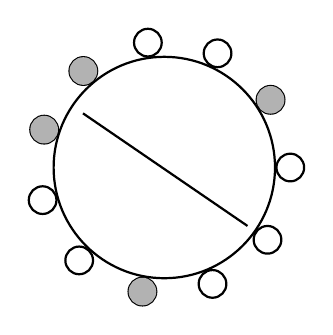
\begin{tikzpicture}[node distance =15em,>=stealth, thick] 
			\node[circle,minimum size =8em, draw, thick] (C){};
			\foreach \i in {0,...,10}\node[circle,minimum size
			=1em,draw,fill=white,thick]at(\i*32.5: 1.6) (\i){};
			\node[circle,minimum size =1em,fill=gray!60]at(4*32.5: 1.6) (17){};
			%\node[]at(7*36: 1.65) (1721){{$r_1$}};
			\node[circle,minimum size =1em,fill=gray!60]at(5*32.5: 1.6) (17){};
			%\node[]at(9*36: 1.65) (1721){{$r_2$}};
			\node[circle,minimum size =1em,fill=gray!60]at(1*32.5: 1.6) (18){}; 
			%\node[]at(2*36: 1.6) (181){{$r_3$}}; 
			\node[circle,minimum size =1em,fill=gray!60]at(8*32.5: 1.6) (29){};
			%\node[]at(4*36: 1.65) (191){{$r_4$}}; 
			
			\node[]at(4.5*32.5: 1.4) (i){};
			\node[]at(10*32.5: 1.45) (ii){};
			\draw (i) -- (ii);

			

			\end{tikzpicture}
	}\hspace{0.5em}
\subfloat[][periodic
	]{
			\centering 
			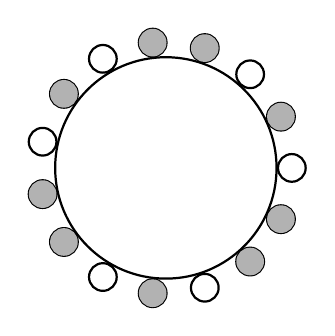
\begin{tikzpicture}[node distance =15em,>=stealth, thick] 
			\node[circle,minimum size =8em, draw, thick] (C){};
			\foreach \i in {0,...,14}\node[circle,minimum size
			=1em,draw,fill=white,thick]at(\i*24: 1.6) (\i){};
					
			\node[circle,minimum size =1em,fill=gray!60]at(3*24: 1.6) (1){};
			\node[circle,minimum size =1em,fill=gray!60]at(4*24: 1.6) (1){};
			\node[circle,minimum size =1em,fill=gray!60]at(6*24: 1.6) (2){};
			\node[circle,minimum size =1em,fill=gray!60]at(8*24: 1.6) (3){};
			\node[circle,minimum size =1em,fill=gray!60]at(9*24: 1.6) (3){};
			\node[circle,minimum size =1em,fill=gray!60]at(11*24: 1.6) (4){};
			\node[circle,minimum size =1em,fill=gray!60]at(13*24: 1.6) (5){};
			\node[circle,minimum size =1em,fill=gray!60]at(14*24: 1.6) (5){};
			\node[circle,minimum size =1em,fill=gray!60]at(1*24: 1.6) (6){};

					

			\end{tikzpicture}
	}
	\caption{Particular configurations}
	\label{fig:introEx}
\end{figure}

\end{example}


The gathering problem on a ring was first investigated by Klasing \textit{et al.}~\cite{KlasingMP06}.
%impossibility results in Fsync
They prove that gathering 2 robots is impossible on any ring, and gathering any number $k > 2 $ robots is impossible without additional assumptions. Proofs of these impossibility results are similar to those in the plane.
A more specific impossibility result is that even if robots are endowed with multiplicity detectors, gathering is impossible for a particular 
class of symmetric configurations. In the sequel we only discuss results given in the Async model.
%explication periodic
%explication edge-edge

In Async, when robots are endowed with weak global multiplicity detectors, %if initial configurations does not contain any multiplicity, the gathering problem is simpler because it is sufficient for a protocol to ensure that a single multiplicity point exists to have all robots gather in this point, so it reduces the gathering problem to the creation of a single multiplicity point. 
the proposed protocols either exploit the symmetries~\cite{klasing_taking_2008} or try to avoid them, and break them when encountered~\cite{KlasingMP06}.
In~\cite{KlasingMP06} the protocol handles only an odd number of robots and starts from any tower-free configuration that is not periodic. 
 %The idea of the proposed solution was to create a single multiplicity which will be the gathering node.
In~\cite{klasing_taking_2008}, the authors provide an algorithm for gathering 18 or more robots on the ring, from any initial configuration not concerned by the impossibility results.
For these initial configurations and less than 18 robots, a number of ring gathering algorithms have been proposed in the literature~\cite{navarrasirocco2011,navarradisc2012,navarraipdps2013,navarrasirocco2013}. They apply to various cases according to 
the size of the ring, the number of robots and the subclass of initial configurations. When multiplicity detection is available a unified 
strategy was proposed in~\cite{navarradisc2012}. 
%In~\cite{ASN11c} the authors address the problem of 6 robots and provide a distributed algorithm that gathers the robots when starting from any symmetric configuration of type node-edge, or node-node.

%%25=
%%23=
%Most of the cases with 4 robots have been solved in [25]. The cases left open in [25], referred to as the set SP4, are symmetric configura- tions of type node–edge with 4 robots and the odd interval cut by the axis bigger than the even one, with an interval being a maximal set of empty consecutive nodes. In general, configurations in SP4 are ungatherable as outlined in [23] for configurations of 4 robots on a five nodes ring. Actually, spe- cific configurations in SP4 could be gatherable but requiring suitable strategies difficult to be generalized. The main diffi- culty faced when dealing with configurations in SP4 comes from the fact that among the two intervals cut by the axis, the odd one is bigger than the even one.

%robots avec local multiplicity detectors
In~\cite{IIKO10c, KLOT11, KLOT12} the authors achieve similar results with weak local multiplicity (robots are not able to see nodes that contain multiple robots unless it is their current node). 
The algorithm by Izumi \textit{et al.}~\cite{IIKO10c} assumes that initial configurations are neither symmetric nor periodic, and the number of robots is less than half the number of nodes. 
For an odd number of robots, %or odd number of nodes in the same model, 
Kamei \textit{et al.}~\cite{KLOT11} propose an algorithm that also works from initial symmetric configurations. 
For an even number of robots on an odd-sized ring, Kamei \textit{et al.}~\cite{KLOT12} propose an algorithm for non periodic initial configurations. %are not periodic. % il y a encore le papier~\cite{navarra2014} des algo pour des conf init particuliéres maid rien d'unifié
An algorithm that achieves the gathering for any initial configuration (when it is possible) is presented in~\cite{DAngeloSN14}: 
it uses existing algorithms as subroutines for the basic solvable cases with 4 or 6 robots from~\cite{4Rob} and~\cite{ASN11c} respectively.

%robots with labels or tokens
%-> similaire à de la communication ou de la mémoire on ne s'en occupe pas

%%limited visibility
%Gathering Asynchronous Oblivious Agents with Local Vision in Regular Bipartite Graphs: In [GP11], the authors studied the gathering problem considering robots having only a local visibility i.e., they can only see robots located at its own and at adjacent nodes. Under this assumption, the authors provide a complete solution of the gathering problem for regular bipartite graphs. They first characterize the class of initial configurations allowing to solve the gathering problem on such graphs, and they propose a gathering algorithm assuming that the system starts from a configuration in this class.
%B. Degener, B. Kempkes, T. Langner, F. Meyer auf der Heide, P. Pietrzyk, and R. Wattenhofer. A tight runtime bound for synchronous gathering of autonomous robots with limited visibility. In Proc. of the 23rd ACM Symp. on Parallelism in algorithms and architectures (SPAA), pages 139–148, 2011.

%%other
%Multiple Agents RendezVous in a Ring in Spite of a Black Hole
%Stefan Dobrev,(black holes) Paola Flocchini, Giuseppe Prencipe, Nicola Santoro
 

\subsection{Exploration}
Exploration is the process by which every location of a \emph{discrete} environment is visited by at least one robot. 
%Due to its definition it must take place in the discrete environment. 
The proposed algorithms mostly try to obtain a common sense of orientation:  the intuition is to arrange the robots in a particular shape, which will allow them to have a common sense of direction, and then to define a direction to explore successfully their environment.
%Like the gathering, the exploration is impossible if the initial configuration is periodic~\cite{flocchini_computing_2007}.
The problem of exploration has several variants, among them the exploration with stop and the perpetual exploration problem.
Both problems are unsolvable if the initial configuration is periodic~\cite{flocchini_computing_2007}.

The study of the exploration begins with the exploration with stop~\cite{flocchini_computing_2007}: 
Robots achieve an exploration with stop if regardless of their initial location, the robots reach a configuration in which they all remain idle and 
each node has been visited by a robot. The difficulty of this task arises from the fact that robots need to stop after all locations have been explored. It requires robots to “remember” how much of the graph was explored: Since they have no persistent memory, this means that they must be able to distinguish between various stages of the exploration process. 
 
Exploration with stop has been studied for paths~\cite{FlocchiniIPS11}, trees~\cite{FlocchiniIPS10}, grids~\cite{devismes_optimal_2011}, rings~\cite{flocchini_computing_2007} and general graphs~\cite{ChalopinFMS10}.
We focus again here on ring topologies, where the problem was studied only for robots endowed with strong global multiplicity sensors.
Flocchini is the first to study this problem in a ring~\cite{flocchini_computing_2007}, she presents an algorithm that permits the exploration with stop for any $k \geq 17$ robots starting from any configuration without multiplicity and where the size of the ring and the number of robots are coprime. The idea is that if $n$ and $k$ are coprime then no periodic configuration can happen.
 Devisme \textit{et al.}~\cite{devismes_optimal_2010-1} prove that there is no exploration protocol (even probabilistic) of an $n$-node ring with three robots for every $n > 3$. 
 Moreover, there exists no deterministic protocol that can explore an even sized ring with $k \leq 4$ robots~\cite{lamani_optimal_2010}: 5 robots are necessary and sufficient when the ring size is even, and 5 robots are sufficient when the size of the ring is odd.
 In~\cite{lamani_optimal_2010} the authors also propose an Async algorithm for 5 robots in an $n$-node ring where $n$ is coprime with five. The proposed algorithm is optimal in the number of robot moves.  
 
 Probabilistic algorithms for the exploration with stop have been studied by Devismes \textit{et al.}~\cite{devismes_optimal_2010-1}.
 This work shows that four identical probabilistic robots are necessary and sufficient in the Ssync model, also removing the coprime constraint between the number of robots and the size of the ring.  A probabilistic protocol is given for $4$ robots to explore any ring of size at least $4$, and a proof that no protocol exists with three robots is given.
 
 %limited visibility
 The case where robots with limited visibility explore an $n$-size ring has been studied by Datta \textit{et al.}~\cite{DattaLLP13}.
When robots have a visibility of 1, the exploration problem is not solvable with deterministic algorithms in Ssync (hence in Async). Even in Fsync, the exploration problem cannot be solved with less than 5 robots when the ring size is more than 6. 
 When they have a visibility of 3, no exploration is possible with less than 5 robots and a ring of size at least 13 in Ssync (and Async).
 In these conditions where the visibility is limited, several algorithms are proposed: 
 \begin{itemize}
 \item Two solutions in the Fsync model, when the visibility is 1: with a minimal number of robots for $3 \leq n \leq 6$ and for $n > 6$.
 \item Two solutions in the Async model, when the visibility is 2: with $7$ robots (for $n > 7$) and $9$ robots (for $n >19$).
 \item  Two solutions in the Async model, when the visibility is 3, with $5$ and $7$ robots.
 \end{itemize}
 %All algorithms work assuming that each robot is at distance at most φ of another one. Both solutions for 7 robots with φ = 2 and 5 robots with φ = 3 work starting from specific configurations.~\cite{exploration with oblivious myopic robots}


%\subsubsection{Exclusive perpetual exploration}
%Perpetual exclusive graph searching: Given a n-node graph G where all edges are contaminated, the graph searching problem consists in coordinating a team of robots to eventually clear all edges. The robots occupy the nodes of G and a robot can move along an edge from its current position to a neighboring node. An edge is cleared by a robot when it traverses it or if both its ends are simultaneously occupied by some robots.
The more difficult problem of exclusive perpetual exploration has been studied recently: 
Robots achieve an exclusive perpetual exploration if regardless of their initial (tower-free) location, each node has been visited by a robot infinitely often and no multiplicity point appears. The latter happens as soon as a moving robot collides with another robot, moving or stationary.
%: this happens when, while moving, it occupies the same location at the same time as another robot. 
 In this context, collisions are considered as undesirable events (with possibly negative consequences), and thus to be avoided. This is expressed by the \emph{exclusivity property}, which states that any node must be occupied by at most one robot.
%Recall that the only time robots are aware of other robots is during the Look phase. In particular, the robots have no way to detect the 
%position of other robots while moving.This means that collision avoidance must be done algorithmically.

Exclusive perpetual exploration has been studied in rings~\cite{blin_exclusive_2010,navarraipdps2013}, grids~\cite{bonnet_asynchronous_2011,baldoni_solvability_2008}, toruses~\cite{devismeshal}, trees~\cite{BlinBN12} and general graphs \cite{baldoni_anonymous_2008,BlinBN13}. 
Blin \textit{et al.}~\cite{blin_exclusive_2010} investigate both the minimal and the maximal number of robots that are necessary and sufficient to solve the exclusive perpetual exploration problem. They also propose algorithms for these two cases:
\begin{itemize}
\item For the lower bound, they prove that 3 robots are necessary and sufficient, provided that the size of the ring is at least 10, and show that no protocol with 3 robots can exclusively perpetually explore a ring of size less than 10. 
\item For the upper bound, they prove that $k = n - 5$ robots are necessary and sufficient to exclusively perpetually explore a ring of size $n$ when $n$ is co-prime with $k$.
\end{itemize}


A more generic algorithm has been proposed in~\cite{navarraipdps2013}: 
starting from any  tower-free configuration that is neither periodic nor symmetric, a ring of size at least $10$ can be perpetually explored by at least $5$ robots. The algorithm does not cover the case of $5$ robots exploring a ring of size $10$. 
% The case where 5 robots want to explore a ring of size 10 is not handled.
Combination of the results in~\cite{blin_exclusive_2010,navarraipdps2013}, leaves open the exclusive perpetual exploration of a ring of general size $n$ by 4 robots.

%Bonnet \textit{et al.} \cite{francois_bonnet_ideal_2012} studied a more difficult version of the exclusive perpetual exploration, 
%where each robot must visit infinitely often all nodes.  
%They prove that sometimes it is impossible even if as a team the robots achieve the perpetual exploration each node is infinitely often visited, 

\bigskip

All the algorithms described above have only been given handmade proofs, some of them rather sketchy. 
In the next section, we present cases where automated proofs were provided.
%Moreover, most of the time only sketches of these proofs have been given. 
%For such critical system the need of for formal verification is well established.

	
%%%%%%%%%%%%%%%%%%%%%%%%%VERIFICATION%%%%%%%%%%%%%%%%%%%%%%%%%%%%%
	\section{Formal Methods for robot algorithms}
Formal methods require mathematical representations of the system and its specification, given as a set of properties.
A distributed system is often described as a global transition system~\cite{Tel:2001:IDA:517021, DBLP:books/mk/Lynch96},
obtained by a composition of models of its sub-systems. 
%The specification can also be expressed by 
 %The set of properties given as its specification. 
 Properties can be classified into various types, among them 
 the well known safety and liveness properties. Safety properties informally require that ``something bad will never happen'', 
 like absence of deadlock. Invariants form an important subclass of safety properties, expressing that ``something is true at every step in every execution''.
 Liveness properties require that ``something good eventually happens'', for example there will be no starvation.
%
%We consider here transition systems for Sub-entities and we use them 
%in this work to represent sub-entities of the system. 
%The complete system is then obtained by a synchronized product of these transition systems. 
%
%Specification of the problem gives the algorithm required properties. for linear-time properties
In the context of linear-time properties, considered in this work, every possible specification can be written as the conjunction of safety and liveness properties~\cite{AlpernS85}.%%%%%%%%%%%%%%%%%%%%%%%%%%%%here%%%%%%%%%%%%%%%%%%%%%%%%%%%%%%%%%%%%%

In this section we present model checking, proof and synthesis, as well as related work for the use of these approaches in the context of 
mobile robot protocols.
		

\subsection{Model checking} \index{Model checking}
A model checker takes as input a model $M$, often in the form of a transition system, describing all possible executions of the system, and the property to be checked, expressed as a logic formula $\varphi$. It answers whether the model satisfies or not the formula. When the property is not satisfied, the model checker returns a counterexample, \textit{i.e.}, an execution of the model invalidating the property. This counterexample is useful to find errors in complex systems. This is an advantage of model checking compared to the other formal methods, such as theorem proving: 
In interactive proofs, one may fail to prove a property without finding out if the property is false or if one just didn't find the proof. 
%Still, some automatic techniques (including satisfiability solving) may be able to disprove a property by constructing a (counter-)model, which %corresponds to a counter-example.%which can disprove a property but without systematically providing such a counterexample. 

%\todo{The automata approach}
The automata approach for model checking was introduced by Vardi \textit{et al.} \cite{vardi_automata-theoretic_1986} to provide a unified and extensible framework, initially applied  to a class of logic formulas called \textsf{LTL} (described later in more details).
This approach splits the verification process of an \textsf{LTL}  formula into three operations: 
\begin{itemize}
\item The language $\mathcal{L} (M)$ associated with $M$ represents all possible executions of $M$. The formula $\varphi$ is translated into an automaton $\mathcal{A}_{\neg \varphi}$ whose language, $\mathcal{L}(A_{\neg \varphi})$, is the set of all executions invalidating $\varphi$.
\item Automata $M$ and $\mathcal{A}_{\neg \varphi}$ are synchronized to obtain an automaton $M \times \mathcal{A}_{\neg \varphi}$ whose language $\mathcal{L}(M \times \mathcal{A}_{\neg \varphi}) = \mathcal{L} (M) \cap  \mathcal{L} (\mathcal{A}_{\neg \varphi})$, is the set of executions of $M$ invalidating $\varphi$.
\item Finally the model checker performs an emptiness check on this product. The model $M$ satisfies $\varphi$ if and only if $\mathcal{L} ( M \times \mathcal{A}_{\neg \varphi}) = \emptyset$. If the emptiness check succeeds, it means that no execution invalidates $\varphi$, hence the property corresponding to $\varphi$ is satisfied by $M$. Otherwise, an execution of $M$ invalidating $\varphi$ is produced as a counterexample.
\end{itemize}		

The drawback of this method is the so-called combinatorial explosion problem~\cite{Valmari96} 
caused by the large size of the product $M \times \mathcal{A}_{\neg \varphi}$. 
The construction of $A_{\neg \varphi}$ is exponential in the size of $\varphi$. Moreover, 
starting from a system of concurrent processes, the automaton $M$ of the system has a size exponential in the number of processes. Consequently, in the automata-theoretic approach the synchronous product is often too large for the emptiness check to be performed in a reasonable execution time and memory.	

Distributed systems are naturally structured as a combination of components, among which several exhibit similar behaviors. Such components are said to be symmetric, and knowing the behavior of one such component is often sufficient to know the behavior of the combination. More formally, the symmetries of the system define an equivalence relation over its states. This relation can be used to produce a reduced state space, where at least one state per equivalence class is kept.
If exactly one representative state per class is kept, then maximal reduction is achieved. The definition of symmetries guarantees that the reduced state space preserves properties, if these properties also cannot distinguish between symmetric executions~\cite{ClarkeJEF96, EmersonS96}. This reduction is usually exponentially smaller than the original state space, thus reducing the execution time and memory of the verification process.

%%%utilisation de its
% Such methods aim to minimize the impact of the graph's size on the performance of model checking algorithms, especially by using concise data structures, like: 
%he state of a distributed system changes when one of its components' state changes.
%Therefore, a given state differs only by a small amount from its immediate neighbors (successors or predecessors).
%An efficient memory representation of such two neighbors should not store twice the common part.
%This motivates the search for efficient data structures that take advantage from the common information in states.
%%	Compact data structures have been developed to represent efficiently large state spaces.
%	The most famous are Decision Diagrams (DD).
%	Introduced by~\cite{bryant1986graph} as a canonical representation for boolean functions, they have then proved successful at representing large sets of states very compactly and efficiently, in particular in the context of model-checking~\cite{burch1992symbolic, fisler2001there, somenzi2002analysis}.
%	Several variants have then be proposed, such as Multi-Valued DD~\cite{srinivasan1990algorithms}, Edge-Valued DD~\cite{lai1992edge} or Data DD (DDD)~\cite{couvreur2002data}.

To our knowledge, in the context of mobile robots operating in discrete space, only one previous attempt, by Devismes \emph{et
  al.}~\cite{devismes_optimal_2011} investigates the possibility of automated verification of mobile robots protocols. They use LUSTRE~\cite{lustre:ieee} to describe and verify the problem of exploration with stop of a $3\times 3$ grid by $3$ robots in the Ssync model.
 They consider particular configurations with a tower of 2 robots and a single robot, where only the single robot wishes to move. 
 For this case, they verify the invariant:  \emph{visited nodes} $\leq 4$. 
	
		\subsection{Proofs}
		%invariant
%hierarchical proof ? je trouve rien de bien a dire ...
%Invariants are mostly proved by induction on the number of steps in the execution.
%So far, the existing proofs of robot protocols operating in the Async model are \emph{ad-hoc} handwritten proofs, that could contain errors.
%Moreover, most of the time only sketches of these proofs have been given.


In mechanical proof assistants, a user can express data, programs, theorems and proofs. Skeptical proof assistants provide an additional guarantee by checking mechanically the soundness of a proof after it has been interactively developed.
They have been successfully employed for various tasks such as the formalization of programming language semantics~\cite{Leroy09}, certification of an OS kernel~\cite{KleinAEHCDEEKNSTW10}, verification of cryptographic protocols~\cite{AlmeidaBBBKB12}, etc.
During the last twenty years, the use of tool-assisted verification has extended to the validation of distributed systems.  


In the mobile robot model described above, mechanical proof assistants provided the certification of impossibility results regarding oblivious and anonymous mobile robots \cite{CourtieuRTU15}, even in presence of Byzantine behaviors \cite{AugerBCTU13}. A certified proof of the impossibility result from~\cite{suzuki_distributed_1999} is proposed in \cite{CourtieuRTU15}, establishing that gathering is impossible with 2 robots. Courtieu \textit{et al.} also provide a more general impossibility result: Gathering with an even number of robots, when the initial position may contain towers is impossible.
		
		\subsection{Synthesis}	 \index{Synthesis}
Going one step further, it is interesting to not only verify or prove some existing algorithms, but to automatically generate an algorithm correct by construction, as done in the synthesis techniques. 
This problem takes as input a specification of a system interacting with an environment, and asks whether there exists a program  satisfying this specification, regardless of the behavior of the environment. When the answer is positive, the program must be effectively built. 
A negative answer gives a proof that there is always a way for the environment to prevent the system from reaching its objective. 

More precisely, let $\varphi$ be the specification that the system must ensure, and let $E$ be a model describing the environment.
The synthesis problem asks whether there exists a program $P$ such that  $P \times E$ satisfies $\varphi$.
The behavior of the system thus created must match exactly all behaviors eligible by the specification. 

It may seem at first that the model actually needed is the one of \emph{distributed games}, in which each robot represents a distinct player, all of them cooperating against a hostile environment. In distributed games, existence of a winning strategy
for the team of players is undecidable \cite{PetersonReif79}. However, the fact that robots are able to see their environment, and thus to always know the configuration of the system, allows us to stay in the framework of 2-player games, and to encode the set of robots as a single player. 
Of course, the strategy obtained will be centralized, but we will design the game in order to obtain only strategies that can be distributed among anonymous, memoryless robots without chirality.
%papier panopticon 

To our knowledge, in the context of mobile robots operating in discrete space, only one previous attempt~\cite{BDPPT12c} investigates the possibility of automated synthesis of mobile robots protocols.
The work considers the exclusive perpetual exploration by $k$ robots of $n$-sized rings in the Ssync model. The approach is brute force: 
it  mechanically generates all \emph{unambiguous} protocols (those that do \emph{not} have symmetric configurations), regardless of the problem to solve, and then checks whether the protocol achieves gathering. 

\bigskip
Following these attempts, we demonstrate in this work a larger use of model checking and synthesis in the context of robot protocols. 
%We show how to apply them to the mobile robots model.
Our approach differs from the previous ones, since our model is general enough to handle all atomicity models, and to accommodate various protocols. Previous works only handle the synchronous models, and apply on specific algorithms. 
%their approaches are restricted to 
%the problem they try to solve. 


	\section{Contributions}
		%\todo{model}
In Chapter~\ref{chap:model} we provide a
formal model for a network of mobile robots operating
under the three execution hypotheses described above, namely Fsync, Ssync
and Async.  We describe the logic \textsf{LTL} (Linear Temporal Logic) used to
specify the requirements corresponding to robot tasks.  Finally, we discuss implementation issues.
%transform this model into the input model of two model-checking tools
%and we prove formally the equivalence of the two models (in terms of
%possible executions).

		%\todo{verif}
The rest of the manuscript presents our contributions and is divided into two parts. In Part~\ref{part:verif} we formally verify two known
protocols for variants of the ring exploration in an asynchronous
setting: exploration with stop from~\cite{flocchini_computing_2007}
and exclusive perpetual exploration
from~\cite{blin_exclusive_2010}. Both protocols were given as 
 informal descriptions in the original papers. This leads us either to a formal correctness proof 
 for particular instances of the analyzed algorithms or to
a counterexample that shows a subtle flaw in the algorithm. 
%For this, we use two model checkers: DiVinE~\cite{Divine13} and
%ITS-tools~\cite{LIP69510}, that offer a convenient input language for
%the translation of automata.
\begin{itemize}
\item  In Chapter~\ref{sec:flo}, we study the case of exploration with stop, and 
more particularly the protocol from~\cite{flocchini_computing_2007}.
  This protocol was manually proved correct
  when the number of robots is $k>17$, and $n$ (the ring size) and $k$
  are coprime. As the necessity of this bound was not proved in the
  original paper, our methodology shows that for many instances
  of $k$ and $n$ not covered in the original paper, the protocol is
  still correct. We offer some conjecture for cases with $k\leq 17$. 
\item Then, in Chapter~\ref{sec:min}, we study the case of the perpetual
  exclusive exploration protocol~\cite{blin_exclusive_2010}. In this
  case, we produce a counterexample in the
   asynchronous setting, where safety is violated. We
  correct the original protocol and verify the new one via
  model checking for several instances of $n$. Additionally, we prove
  the correctness of the protocol for any size of ring with an inductive
  approach.  
\end{itemize}
		%\todo{Synthese}
In Part~\ref{part:synth}, we show how automated synthesis can be applied to generate correct robot protocols, 
in the discrete space model. As a case study, we consider the problem of gathering.
\begin{itemize}
\item In Chapter~\ref{chap:synth}, we propose an encoding of the gathering problem in a synchronous 
execution model as a reachability game, the players being the robot algorithm 
on one side, and the scheduling adversary (that can also dynamically choose 
robot chirality at every activation) on the other side. Our encoding is 
general enough to encompass classical execution models for robots evolving on 
ring-shaped networks, including (and contrary to the existing ad-hoc solution~\cite{BDPPT12c}) 
when several robots are located at the same node and when symmetric situations occur. 
This allows us to automatically generate an \emph{optimal} distributed algorithm, in the Fsync model, 
for three robots evolving on a fixed size ring. Our optimality criterion refers to the number of robot 
moves that are necessary to actually achieve gathering.
\item In Chapter~\ref{chap:asynth}, we consider the asynchronous model. 
We first show how finding an algorithm for gathering asynchronous robots 
can be seen as an extension of two player games, namely games with partial information. 
In these games, contrary to the previous ones, players have an incomplete view of the system.
In order to fight the combinatorial explosion due to the asynchronous model,
we propose a recursive algorithm that permits to obtain a gathering
protocol in this setting, thanks to synchronous 
synthesis combined with model checking. 
\end{itemize}
	
	
	%We first define some notations and models 
	
	
%	\todo{complexity}
%	voir papier fraignaud pelc verifiable decidable ....
%	voir np complet et MAD and MAV
	
%	\todo{dans le modèle dire que le modèle de robots en le modélise comme un ensemble de processus Asynchrones}
	
	